\documentclass[10pt,english,aspectratio=169]{beamer}
% Use notes or hide notes or show only notes or handout


\usetheme{default}

\usepackage{xstring}
\usepackage{pgfpages}
%\makeatletter
%\IfSubStr{\@classoptionslist}{handout}
%  {\pgfpagesuselayout{2 on 1}[letterpaper,border shrink=5mm]}
%  {}
%\makeatother

\usepackage{amsmath,amssymb,amsthm}
\usepackage{stmaryrd}
\usepackage{enumerate}
\usepackage{stfloats}
\usepackage{bbm}
\usepackage{pdfpages}
\usepackage{framed}

\usepackage[most]{tcolorbox}
\tcbset{highlight math style={enhanced,
  colframe=white,colback=yellow!15,arc=8pt,boxrule=1pt,
  }}
  
\usepackage{tikz,pgf,pgfplots}
\usepackage{algorithm,algorithmic}
\usepgflibrary{shapes}
\usetikzlibrary{%
  arrows,%
  arrows.meta,
  shapes.misc,% wg. rounded rectangle
  shapes.arrows,%
  shapes,%
  calc,%
  chains,%
  matrix,%
  positioning,% wg. " of "
  scopes,%
  decorations.pathmorphing,% /pgf/decoration/random steps | erste Graphik
  shadows,%
  backgrounds,%
  fit,%
  petri,%
  quotes
}

\setbeamersize{text margin left=10mm,text margin right=35mm}

\pgfplotsset{compat=1.12}

%\usetheme{Frankfurt}
%\usecolortheme{ldpc}
\useinnertheme{rounded}
\usecolortheme{whale}
\usecolortheme{orchid}

\newcommand{\ul}[1]{\underline{#1}}
\renewcommand{\Pr}{\mathbb{P}}

%% Setup slides and notes
\makeatletter
\IfSubStr{\@classoptionslist}{notes} { \IfSubStr{\@classoptionslist}{hide} {}{\IfSubStr{\@classoptionslist}{only} {}{\setbeameroption{show notes on second screen=right}}} }{}
\makeatother
%\setbeamertemplate{note page}{\pagecolor{yellow!5}\vfill\insertnote\vfill}

\newcommand{\getpdfpages}[2]{\begingroup
  \setbeamercolor{background canvas}{bg=}
  \addtocounter{framenumber}{1}
  \includepdf[pages={#1},%
  pagecommand={%
    \expandafter\def\expandafter\insertshorttitle\expandafter{%
      \insertshorttitle\hfill\insertframenumber\,/\,\inserttotalframenumber}}%
  ]{#2}
  \endgroup}

\newcommand{\backupbegin}{
   \newcounter{finalframe}
   \setcounter{finalframe}{\value{framenumber}}
}
\newcommand{\backupend}{
   \setcounter{framenumber}{\value{finalframe}}
}

 \setbeamercolor{bibliography entry author}{fg=black}
 \setbeamercolor{bibliography entry title}{fg=black}
 \setbeamercolor{bibliography entry location}{fg=black}
 \setbeamercolor{bibliography entry note}{fg=black}
 
 \setbeamerfont{bibliography item}{size=\footnotesize}
 \setbeamerfont{bibliography entry author}{size=\footnotesize}
 \setbeamerfont{bibliography entry title}{size=\footnotesize}
 \setbeamerfont{bibliography entry location}{size=\footnotesize}
 \setbeamerfont{bibliography entry note}{size=\footnotesize}
 \setbeamertemplate{bibliography item}{\insertbiblabel}
 
\newlength\tikzwidth
\newlength\tikzheight


\newcommand{\mc}[1]{\mathcal{#1}}
\newcommand{\mbb}[1]{\mathbb{#1}}
%\newcommand{\expt}{\mbb{E}}
%\newcommand{\dd}{\mathrm{d}}
%\usepackage{fixltx2e}

\newcommand{\Interior}[1]{\ensuremath{{#1}^{\circ}}}
\newcommand{\Closure}[1]{\ensuremath{\overline{#1}}}
\newcommand{\Complement}[1]{\ensuremath{{#1}^{c}}}

\newcommand{\Expect}{\ensuremath{\mathrm{E}}}
\newcommand{\vecnot}{\underline}
\newcommand{\RealNumbers}{\mathbb{R}}
\newcommand{\RationalNumbers}{\mathbb{Q}}
\newcommand{\ComplexNumbers}{\mathbb{C}}
\newcommand{\Real}{\mathrm{Re}}
\newcommand{\Span}{\mathrm{span}}
\newcommand{\Rank}{\mathrm{rank}}
\newcommand{\Nullity}{\mathrm{nullity}}
\newcommand{\Trace}{\mathrm{tr}}
\newcommand{\Diag}{\mathrm{diag}}
\DeclareMathOperator*{\esssup}{ess\,sup}
\newcommand{\dd}{\mathrm{d}}



\def\checkmark{\tikz\fill[scale=0.4](0,.35) -- (.25,0) -- (1,.7) -- (.25,.15) -- cycle;}
\def\greencheck{{\color{green}\checkmark}}
\def\scalecheck{\resizebox{\widthof{\checkmark}*\ratio{\widthof{x}}{\widthof{\normalsize x}}}{!}{\checkmark}}
\def\xmark{\tikz [x=1.4ex,y=1.4ex,line width=.2ex, red] \draw (0,0) -- (1,1) (0,1) -- (1,0);}
\def\redx{{\color{red}\xmark}}

\renewcommand{\footnotesep}{-2pt}


\begin{document}



\title{ECE 586: Vector Space Methods \\ Lecture 5 Flip Video: Metric Spaces and Topology}
\author{Henry D. Pfister \\ Duke University}
\date{}
%\date{August 20th, 2020}
%\maketitle

\setbeamertemplate{navigation symbols}{}

\begin{frame}[plain]
	\titlepage
	
	\note{
		\vspace{8mm}
		\begin{enumerate}
			\setlength\itemsep{3mm}
			\color{red}
			\item Welcome to the fifth video lecture for ECE 586, Vector Space Methods. \\[2mm]
			Today, we'll discuss metric spaces and topology.
		\end{enumerate}
	}
\end{frame}

\addtocounter{framenumber}{-1}
\setbeamertemplate{navigation symbols}{\textcolor{blue}{\footnotesize \insertframenumber ~/ \inserttotalframenumber}}

\begin{frame}<1-6> \frametitle{2.1: Introduction}

\begin{itemize}
\setlength\itemsep{3mm}
\item<1-> What is topology and why do we study it? \vspace{1mm}
\begin{itemize} 
  \setlength\itemsep{1.5mm}
  \item<1-> \textcolor{blue}{Study of geometric properties preserved by continuous deformations}
  \item<2-> Why? Engineers approximate real things by mathematical objects
  \item<2-> Q1: Can a matrix $A$ be approximated closely by a lower rank matrix?
  \item<2-> Q2: Can a function $f(x)$ be approximated well by a degree-2 polynomial?
  \item<3-> In engineering, a topology is typically defined using a metric
\end{itemize}

\vspace{1mm}

\item<4-> Metric Spaces \vspace{1mm}
\begin{itemize} 
  \setlength\itemsep{1.5mm}
  \item<4-> A \textcolor{blue}{metric space} $(X,d)$ is a set $X$ along with a metric $d(x,y)\!\!$
  \item<4-> $d(x,y)$ is called the \textcolor{blue}{distance} between the \textcolor{blue}{points} $x$ and $y$
  \item<5-> A \textcolor{blue}{metric} on a set $X$ is a function \textcolor{blue}{$d \colon X \times X \rightarrow \mathbb{R} $} such that: \vspace{1mm}
  \begin{itemize}
  \setlength\itemsep{1.5mm}
  \item<5->[1.] $d(x,y) \geq 0 \quad \forall x, y \in X$; with equality iff $x = y$ \hfill (non-negativity)~~~~~~~~~
  \item<5->[2.] $d(x,y) = d(y,x) \quad \forall x, y \in X$ \hfill (symmetry)~~~~~~~~~
  \item<6->[3.] $d(x,y) + d(y,z) \geq d(x,z) \quad \forall x, y, z \in X$ \hfill (triangle inequality)~~~~~~~~~
  \end{itemize}
\end{itemize}
\end{itemize}

\begin{tikzpicture}[overlay,remember picture,shift={(12.5,1.5)}]
\uncover<4->{%
	\draw[fill=blue!10] (-1,-1) rectangle (2.2,1.2); 
    \node at (1.7,0.6) {$X$};
    \node[circle,label={$x$},fill=black,minimum size=3pt, inner sep=0pt] (a) at (-0.55,0.3) {};
    \node[circle,label={$z$},fill=black,minimum size=3pt, inner sep=0pt] (c) at (1.7,-0.4) {};
    \draw (a) -- (c) node[blue,midway,above,sloped] {$d(x,z)$};
}
\uncover<6->{%
    \node[circle,label=below:{$y$},fill=black,minimum size=3pt, inner sep=0pt] (b) at (0.05,-0.45) {};
    \draw (a) -- (b) node[blue,midway,below,sloped] {$d(x,y)$};
    \draw (b) -- (c) node[blue,midway,below,sloped] {$d(y,z)$};
}
\end{tikzpicture}

\note{
	\vspace{2mm}
	\begin{enumerate}[<alert@+>]
		\footnotesize
		\setlength\itemsep{3mm}
		\item Read.  It allow one to define abstract notions of proximity and distance.
		\item Why do we study it? Read. Here are two questions that it can help answer. 
		\item Read.  Thus, this course will focus on metric spaces.
		\item Read.  This definition provides is a useful abstraction of spaces with some notion of distance between any two points.
		\item Read.  These rules can be seen as an abstraction of Euclidean space whose notion of distance retains some key properties of Euclidean distance.
		\item Read. For example, suppose $x$ is where you work, $z$ is where you live, and $y$ is where you buy groceries.  Then, the triangle inequality abstracts the idea that stopping by the store on your way home cannot make your trip home shorter.
	\end{enumerate}
}

\end{frame}


\begin{frame}<1-3> \frametitle{2.1: Standard Examples of Metric Spaces}

\begin{itemize}
\setlength\itemsep{6mm}
\item<1-> Real numbers $X=\mathbb{R}$ with \textcolor{blue}{absolute distance} $d(x,y)=|x-y|$ \vspace{1mm}
\begin{itemize} 
  \setlength\itemsep{1.5mm}
  \item Foundation for real analysis: 1. and 2. are easy; 3. follows from \[ |x-z| = |(x-y) + (y-z)| \leq |x-y| + |y-z| \]
\end{itemize}

\item<2-> $X=\mathbb{R}^n$ with \textcolor{blue}{Euclidean metric $d(\vecnot{x},\vecnot{y})=\sqrt{(x_1-y_1)^2 + \ldots + (x_n-y_n)^2}\!\!\!\!\!\!$}\vspace{1mm}
\begin{itemize} 
  \setlength\itemsep{1.5mm}
  \item Properties 1. and 2. are easy; 3. is a bit harder and will be shown later
\end{itemize}

\item<3-> Continuous functions $f \colon [a,b] \to \mathbb{R}$ with metric \textcolor{blue}{$d(f,g) = \displaystyle{\max_{x\in [a,b]}} | f(x) - g(x) |\!\!\!\!\!\!\!\!\!\!\!\!\!\!\!\!\!\!\!\!\!$}\vspace{0.5mm}
\begin{itemize} 
  \setlength\itemsep{1.5mm}
  \item Properties 1. and 2. \textcolor{blue}{inherited} from absolute distance; 3. follows from
  \begin{align*}
    \max_{x\in [a,b]} | f(x) - h(x) |
    &= \max_{x\in [a,b]} | f(x) - g(x) + g(x) - h(x) |  \\
    &\leq \max_{x\in [a,b]} \left[ |f(x) - g(x)| + |g(x) - h(x)| \right] \\
    &\leq \max_{x\in [a,b]} |f(x) - g(x)| + \max_{x\in [a,b]} |g(x) - h(x)| = d(f,g) + d(g,h)
  \end{align*}
\end{itemize}

%\item<3-> Real vectors $X=\mathbb{R}^n$ with metric \textcolor{blue}{$d(\vecnot{x},\vecnot{y}) \triangleq \max \{|x_1 - y_1|,\ldots,|x_n - y_n|\}$} \vspace{1mm}
%\begin{itemize} 
%  \setlength\itemsep{1.5mm}
%  \item Properties \textcolor{blue}{inherited} from absolute distance: 1. and 2. easy; 3. from
%  \begin{align*}
%    \max \{|x_1 - z_1|,\ldots,|x_n - z_n|\}
%    &= \max \{|x_1 - y_1 + y_1 - z_1|,\ldots,|x_n - y_n + y_n -z_n|\} \\ 
%    &\leq \max \{|x_1 - y_1| + |y_1 - z_1|,\ldots,|x_n - y_n| + |y_n -z_n|\} \\
%    &\leq \max \{|x_1 - y_1|,\ldots,|x_n - y_n|\} + \max \{|y_1 - z_1|,\ldots,|y_n -z_n|\}
%  \end{align*}
%\end{itemize}

\end{itemize}

\note{
	\vspace{2mm}
	\begin{enumerate}[<alert@+>]
		\footnotesize
		\setlength\itemsep{3mm}
		\item First, consider the (read).  This example is the standard (read). 1 holds because the absolute value of a number is non-negative and equals zero iff that number is zero.  2 holds because swapping $x,y$ doesn't change the absolute value. Read.
		\item Next, consider the example of real $n$-dimensional vectors (read).
		\item Finally, consider the set of (read).  For this metric, many of the properties are inherited from the absolute distance inside the maximum.  In particular, properties 1 and 2 follow naturally.  For the triangle inequality, we observe that: \\ [2mm] (a) the absolute difference between $f(x)$ and $h(x)$ is unchanged by adding and subtracting $g(x)$ inside the absolute value, \\ [2mm] (b) the absolute value of the sum of two numbers is upper bounded the sum of their absolute values, \\ [2mm] (c) the maximum of the sum of two functions is only increased by maximizing them separately.
	\end{enumerate}
}

\end{frame}

\begin{frame}<1-3> \frametitle{2.1: Important Concepts in Metric Spaces}

\begin{itemize}
\setlength\itemsep{5mm}
\item<1-> \textcolor{red}{``Set of points with distance less than $\epsilon$ from a point $x$''} \vspace{1mm}
\begin{itemize} 
  \setlength\itemsep{1.5mm}
  \item This is called the \textcolor{blue}{open ball} of radius $\epsilon$ centered at $x$ and given by \vspace{-1mm} \[\color{blue} B_d(x,\epsilon) \triangleq \left\{ y \in X | d(x,y) < \epsilon \right\} \vspace{-5mm} \]
  \item $P=$``For all $a\!\in\! B_d (x,\epsilon)$, there is $\delta\!>\!0$ s.t. $B_d (a,\delta) \subseteq B_d (x,\epsilon)$''
\end{itemize}

\item<2-> \textcolor{red}{``Infinite list $x_1,x_2,x_3,\ldots$ of points in $X$''} \vspace{1mm}
\begin{itemize} 
  \setlength\itemsep{1.5mm}
  \item A \textcolor{blue}{sequence} $x_i \in X$ for $i\in \mathbb{N}$ equivalent to $x_i = f(i)$ for $f:\mathbb{N}\to X$
  \item Ex. For $X=\mathbb{R}$ and $d(x,y)=|x-y|$, let \textcolor{blue}{$x_n = \left(1+\frac{1}{n}\right)^n$} for $n\in \mathbb{N}$
\end{itemize}

\item<3-> \textcolor{red}{``A sequence of points that approaches another point''} \vspace{1mm}
\begin{itemize} 
  \setlength\itemsep{1.5mm}
  \item A sequence $x_n$ \textcolor{blue}{converges} to $x\in X$ (denoted \textcolor{blue}{$x_n \to x$})  if, for any $\epsilon >0$, there is natural number $M$ such that $d(x,x_n) < \epsilon$ for all $n>M$
\end{itemize}
  
\end{itemize}

\begin{tikzpicture}[overlay,remember picture,shift={(11.5,0)}]
\uncover<1>{%
\draw[very thick] (0,0) rectangle (3,2.75) node[below left=0.2cm and 0.2cm] {$X$};
\draw[thick,dashed,blue,fill=blue!10] (0.7,1.6) circle (0.6) node[above=0.55cm] {$B_d(x,\epsilon)$};
\node [label=below:{$x$},draw,fill=black,circle,inner sep=0pt,minimum size=3pt] at (0.7,1.6) {};
\draw[-latex] (0.7,1.6) -- node[above] {$\epsilon$} (0.1,1.6);
}
\uncover<2->{%
\draw[very thick] (0,0) rectangle (3,2.75) node[below left=0.2cm and 0.2cm] {$X$};
\foreach \i/\x/\y in {1/27/6,2/22/11,3/18.5/13.5,4/15/15} {%
\node [label=below:{$x_\i$},draw,fill=black,circle,inner sep=0pt,minimum size=3pt] (x\i) at (\x/10,\y/10) {};
1.25,1.25) {}; }
\node at (1.1,1.56) {\ldots};
}
\uncover<3->{%
\node [label=below:{\textcolor{blue}{$x$}},draw,fill=blue,circle,inner sep=0pt,minimum size=3pt] (x) at (0.7,1.6) {};
}
\end{tikzpicture}

\note{
	\vspace{8mm}
	\begin{enumerate}[<alert@+>]
		\footnotesize
		\setlength\itemsep{3mm}
		\item First, let us consider the (read).  This is illustrated in the figure.  Also, the statement denoted $P$ (read) says that all points in the open ball of radius $\epsilon$ also have an open ball around them of radius $\delta < \epsilon$ that lies entirely inside the original ball.  You will be asked to prove this in the homework.
		\item Next, consider an (read).  Formally, we say that (read). It is well-known that this sequence converges to the constant $e$. A sequence is also illustrated in figure.
		\item Finally, consider (read).  Formally, we say that (read). In the figure, one can imagine the example sequence converging to the point $x$.
	\end{enumerate}
}

\end{frame}


\begin{frame}<1-5> \frametitle{2.1: Convergence: Examples and Counterexamples}

\begin{definition}<1->
A sequence $x_1,x_2,\ldots$ in $(X,d)$ is a \textcolor{blue}{Cauchy sequence} if, for any $\epsilon >0$, there is a natural number $N$ (which may depend on $\epsilon$) such that, for all $m,n > N$,\vspace{-2mm}
\begin{equation*}
d \left( x_m, x_n \right) < \epsilon
\end{equation*}
\end{definition}

\begin{itemize}
\setlength\itemsep{3mm}
\item<2-> Theorem: Every convergent sequence is a Cauchy sequence \vspace{1mm}
\begin{itemize} 
  \setlength\itemsep{1.5mm}
  \item Proof will be given in the lecture \pause
\end{itemize}
\item<3-> Converse? \uncover<4->{No, there is a counterexample} \vspace{1mm}
\begin{itemize} 
  \setlength\itemsep{1.5mm}
  \item<4-> Metric space $(X,d)$ with rationals $X=\mathbb{Q}$ and $d(x,y)=|x-y|$
  \item<4-> Sequence $x_1 = 2$ and $x_{n+1} = f(x_n) \triangleq \frac{1}{2} x_n + 1/x_n \in \mathbb{Q} $
  \item<4-> One can show: $x_n$ is a Cauchy sequence and $|x_n - \sqrt{2}|\to 0$
\end{itemize}
\item<5-> But, according to the definitions, \textcolor{blue}{$x_n$ does not converge!}  \vspace{1mm}
\begin{itemize} 
  \setlength\itemsep{1.5mm}
  \item Because convergence requires that the limit is in $X$ but $\sqrt{2} \notin \mathbb{Q}$
\end{itemize}
\end{itemize}

\note{
	\vspace{4mm}
	\begin{enumerate}[<alert@+>]
		\footnotesize
		\setlength\itemsep{3mm}
		\item Read.  For the real numbers, you've probably seen this definition before in a calculus class.
		\item Read.  This means that the tail of a convergent sequence must only contain points that are close to each other.
		\item What about the converse? In calculus and real analysis, it is also common to prove convergence by showing a sequence in Cauchy.
		\item But this doesn't work in all metric spaces! Read.
		\item Read.  Thus, this counterexample follows from the irrationality of $\sqrt{2}$.  Later, we will see that the converse is true for complete metric spaces.
	\end{enumerate}
}

\end{frame}

  
\begin{frame}<1-3> \frametitle{2.1.1: Metric Topology}

\begin{definition}<1->
Let $W$ be a subset of a metric space $(X,d)$.
The set $W$ is called \textcolor{blue}{open} if, for every $w_0 \in W$, there is an $\epsilon>0$ such that $B_d (w_0,\epsilon) \subseteq W$.
\end{definition}

\begin{definition}<2->
A subset $W$ of $(X,d)$ is \textcolor{blue}{closed} if its complement $W^c = X-W$ is open.
\end{definition}

\begin{theorem}<3->
%For any metric space $(X,d)$,
\begin{enumerate}
\item $\emptyset$ and $X$ are open sets
\item any union of open sets is open
\item any finite intersection of open sets is open
\end{enumerate}
\end{theorem}

\begin{center}
\scalebox{0.7}{%
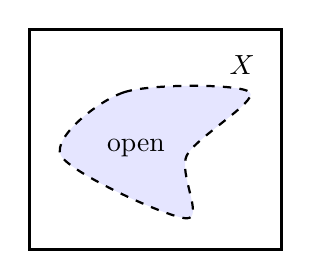
\begin{tikzpicture}[scale=0.8]
\draw[very thick] (-0.5,-1.5) rectangle (3.5,2) node[below left=0.2cm and 0.2cm] {$X$};
\draw [thick,dashed,fill=blue!10] plot [smooth cycle] coordinates {(0,0) (1,1) (3,1) (2,0) (2,-1)} node[above left=0.65cm and 0.15cm] {open};
\end{tikzpicture}}
\hspace{5mm}
\scalebox{0.7}{%
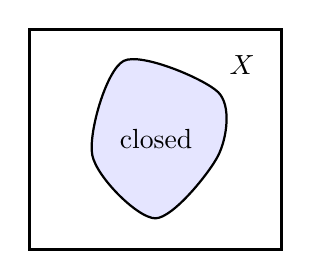
\begin{tikzpicture}[scale=0.8]
\draw[very thick] (-0.5,-1.5) rectangle (3.5,2) node[below left=0.2cm and 0.2cm] {$X$};
\draw [thick,fill=blue!10] plot [smooth cycle] coordinates {(0.5,0) (1,1.5) (2.5,1) (2.5,0) (1.5,-1)} node[above left=0.75cm and -0.6cm] {closed};
\end{tikzpicture}}
\hspace{5mm}
\scalebox{0.7}{%
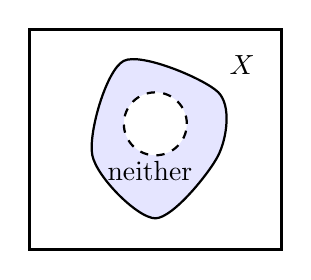
\begin{tikzpicture}[scale=0.8]
\draw[very thick] (-0.5,-1.5) rectangle (3.5,2) node[below left=0.2cm and 0.2cm] {$X$};
%\clip (1,1) circle(0.5);
\fill[blue!10,even odd rule] plot [smooth cycle] coordinates {(0.5,0) (1,1.5) (2.5,1) (2.5,0) (1.5,-1)} (1.5,0.5) circle (0.5);
\draw[thick,dashed] (1.5,0.5) circle (0.5);
\draw [thick] plot [smooth cycle] coordinates {(0.5,0) (1,1.5) (2.5,1) (2.5,0) (1.5,-1)} node[above left=0.35cm and -0.6cm] {neither};
\end{tikzpicture}}
\end{center}  

\note{
	\vspace{4mm}
	\begin{enumerate}[<alert@+>]
		\footnotesize
		\setlength\itemsep{3mm}
		\item In mathematics, a topology is a collection of ``open'' sets satisfying certain properties. It's likely that many of you have been exposed informally to the idea of open and closed sets (e.g., intervals of real numbers).  In this class, we will make these notions precise for metric spaces.   Read.
		\item Read.
		\item Based on these definitions, one can prove the following theorem. Read. These results will be proven in class or in homework problems.
	\end{enumerate}
}

\end{frame}


\begin{frame}<1-6> \frametitle{2.1.1: Interior, Limit points, and Closure}

For a metric space $(X,d)$ and subset $W \subseteq X$:

\begin{definition}<1->
A point $w_0 \in W$ is in the \textcolor{blue}{interior} of $W$ (denoted $\Interior{W}$) if: \\ ~~there is a $\delta >0$ such that $B_d (w_0,\delta) \subseteq W$. %if $d(x,w)<\delta$, then $x\in W$.
\end{definition}

\begin{definition}<2->
A point $x_0 \in X$ is a \textcolor{blue}{limit point} of $W$ if there is: \\  ~~a sequence of distinct elements, $w_1,w_2,\ldots\in W$, that converges to $x_0$.
\end{definition}

\begin{definition}<3->
A point $x_0\in X$ is in the \textcolor{blue}{closure} of $W$ (denoted $\Closure{W}$) if: \\ ~~for all $\delta >0$, there is a $w_0\in W$ such that $d(x_0,w_0)<\delta$.
\end{definition}

\begin{itemize}
  \setlength\itemsep{1.5mm}
  \item<4-> The interior $\Interior{W}$ is open (see definition)
  \item<5-> $W$ is closed if and only if it contains all of its limit points
  \item<6-> Closure $\Closure{W}$ equals union of $W$ and all its limit points (thus is closed)
\end{itemize}

\note{
	\vspace{4mm}
	\begin{enumerate}[<alert@+>]
		\footnotesize
		\setlength\itemsep{2mm}
		\item Sometimes it is useful to consider only the points in a set that are not part of a boundary.  This is called the interior of the set and for a... Read.  This implies that $w_0$ surrounded by an open ball in $W$.
		\item It is also useful to consider points that can approached by non-trivial sequences from a set. These points are called limit points.  Formally, ... Read.  
		\item It can also be useful to consider a set along with all additional points lying on its boundary.  The resulting set is called the closure and, formally, ... Read.  This implies that $x_0$ is arbitrarily close to points in $W$.
		\item These sets have a few nice properties.  First, one can show that the interior is open.
		\item One can also show that (read).
		\item Lastly, one can show that the (read).
	\end{enumerate}
}


\end{frame}

\begin{frame}<1-2> \frametitle{A Few More Things}

\begin{itemize}
  \setlength{\itemsep}{4mm}
  \item Consider the standard metric space of real numbers $\mathbb{R}$ \vspace{1mm}
  \begin{itemize}
    \setlength{\itemsep}{2mm}
    \item<1-> Any open set can be written as countable disjoint union of open intervals
    \item But, what about closed sets?
    \item In higher dimensions, this fails for any connected set that is not a ball
  \end{itemize}
  
  \item<2-> The Boundary \vspace{1mm}
  \begin{itemize}
    \setlength{\itemsep}{2mm}
    \item For $W \subseteq X$, the \textcolor{blue}{boundary} $\partial W$ is the closure minus the interior $\Closure{W} - \Interior{W}\!\!\!$
    \item Thus, the closure is the union of the set and its boundary
    \item In the figure, the boundary is the union of the dashed and solid lines
    \item Alternatively, a point $x\in X$ is on the \textcolor{blue}{boundary} of $W$ if, for all $\delta>0$, $B_d (x,\delta)$ contains a point in $W$ and a point not in $W$

  \end{itemize}
\end{itemize}

\begin{tikzpicture}[overlay,remember picture,shift={(12.5,0.25)}]
\begin{scope}[scale=0.6]
\uncover<2->{%
\draw[very thick] (-0.5,-1.5) rectangle (3.5,2) node[below left=0.1cm and 0.1cm] {\small $X$};
\fill[blue!10,even odd rule] plot [smooth cycle] coordinates {(0.5,0) (1,1.5) (2.5,1) (2.5,0) (1.5,-1)} (1.5,0.5) circle (0.5);
\draw[thick] (1.5,0.5) +(-80:0.5) arc (-80:80:0.5);
%\draw[thick] (1.5,0.5) arc (-20:40:0.5);
%\path[thick,dashed] (1.5,0.5) coordinate (A) (1.5,0.5) coordinate (B) (60:0.5) coordinate (C) (120:0.5) coordinate (D);
\draw[thick,dashed] (1.5,0.5) circle (0.5);
\draw [thick,dashed] plot [smooth cycle] coordinates {(0.5,0) (1,1.5) (2.5,1) (2.5,0) (1.5,-1)} node[above left=0.1cm and -0.3cm] {\small $W$};
%\path[draw,thick] (0.5,0) --  (1,1.5) --  (2.5,1);
}
\end{scope}

\end{tikzpicture}

\note{
	\vspace{4mm}
	\begin{enumerate}[<alert@+>]
		\footnotesize
		\setlength\itemsep{3mm}
		\item Read to 2nd bullet. For closed sets, De Morgan's law implies that any closed set can be written as the countable disjoint intersection of closed intervals. But, exotic sets like the Cantor set show that they cannot be written as the countable union of closed sets. Read. This is because the disjoint union of multiple open balls cannot be connected.
		\item Read. Thus, boundary points are either in the set and arbitrarily close to points outside the set or outside the set and arbitrarily close to points inside the set.
	\end{enumerate}
}

\end{frame}



\begin{frame} \frametitle{Next Steps}

\begin{itemize}
\setlength\itemsep{5mm}
\item To continue studying after this video -- \vspace{2mm}

\begin{itemize}
 \setlength\itemsep{3mm}
 \item Try the suggested reading: Course Notes EF 2.1-2.1.2
 \item Or the optional reading: MMA 2.1
 \item Also, look at the problems in Assignment 3
\end{itemize}
\end{itemize}

\note{
	\vspace{8mm}
	\begin{enumerate}
		\setlength\itemsep{3mm}
		\color{red}
		\item Here are some options to continue learning this material. (read) \\ [2mm]  That's it for today.  So, I'll see you next time.
	\end{enumerate}
}

\end{frame}

  
\backupbegin

%\begin{frame}
%\frametitle{Backup Slides}
%\begin{itemize}
%\item Slide numbers not included in denominator!
%\end{itemize}
%\end{frame}

%\begin{frame}[allowframebreaks]
%\frametitle{References}
%\bibliographystyle{alpha}
%\footnotesize
%\bibliography{IEEEabrv,WCLabrv,WCLbib,WCLnewbib}
%\end{frame}

\backupend

\end{document}
